\documentclass[a4paper,12pt]{article}

\usepackage{amsfonts, amsmath, amssymb, authblk, scrextend, hyperref, enumerate,mathtools, tikz, csquotes, mathrsfs, lmodern,arydshln, xypic, bbold, graphicx}
\usepackage[mathcal]{eucal}
\usetikzlibrary{matrix}
\usepackage[lmargin=2.5 cm,rmargin=2.5cm,tmargin=3cm,bmargin=3cm]{geometry}

\allowdisplaybreaks
\everymath{\displaystyle}
\setlength\parindent{0pt}

\newcommand{\dlim}{\underset{\longrightarrow}{\lim} \ }
\newcommand{\field}[1]{\mathbb{#1}}
\newcommand{\N}{\field{N}}
\newcommand{\one}{\field{1}}
\newcommand{\disp}{\displaystyle}
\newcommand{\Z}{\field{Z}}
\newcommand{\Q}{\field{Q}}
\newcommand{\F}{\field{F}}
\newcommand{\C}{\field{C}}
\newcommand{\R}{\field{R}}
\renewcommand{\det}[1]{\text{det}\3(#1\4)}
\newcommand{\ind}{\mathbb{1}}
\newcommand{\var}{\text{Var}}
\newcommand{\val}{\text{Val}}
\newcommand{\sd}{\text{SD}}
\newcommand{\cov}{\text{Cov}}
\newcommand{\pr}{\text{Pr}}
\renewcommand{\bf}[1]{\textbf{#1}}
\renewcommand{\it}[1]{\textit{#1}}
\renewcommand{\tt}[1]{\texttt{#1}}
\newcommand{\ul}[1]{\underline{#1}}
\newcommand{\mscr}[1]{\mathscr{#1}}
\newcommand{\spec}{\textbf{spec}}
\newcommand{\A}{\field{A}}
\newcommand{\liff}{\leftrightarrow}
\newcommand{\tr}[1]{\text{trace}\3(#1\4)}
\newcommand{\limf}{\lim_{n \to \infty}}
\newcommand{\3}{\left}
\newcommand{\4}{\right}
\renewcommand{\-}[1]{{}^{-#1}}
\newcommand{\up}[1]{{}^{#1}}
\newcommand{\Id}{\text{Id}}
\newcommand{\cat}[1]{\mathcal{#1}}
\newcommand{\bdiv}{\ \textbf{div} \ }
\newcommand{\bbmod}{\ \textbf{mod} \ }
\newcommand{\Hom}{\text{Hom}}
\newcommand{\Rel}{\text{Rel}}
\newcommand{\id}[1]{\text{id}_{#1}}
\newcommand{\proj}[1]{\text{proj}_{#1}}
\newcommand{\ppmod}[1]{\ (\text{mod $#1$})}
\newcommand{\ceil}[1]{\3\lceil \text{$#1$} \4\rceil}
\newcommand{\floor}[1]{\3\lfloor \text{$#1$} \4\rfloor}
\newcommand{\power}[1]{\mathcal{P}(#1)}
\newcommand{\tri}[1]{\triangle_{#1}}
\newcommand{\inj}{\hookrightarrow}
\newcommand{\im}{\text{Im}}
\newcommand{\edel}{\epsilon-\delta}
\newcommand{\empt}{ \varnothing}
\newcommand{\inv}{^{-1}}
\newcommand{\ideal}[1]{\mathfrak{#1}}
\def\upint{\mathchoice%
    {\mkern13mu\overline{\vphantom{\intop}\mkern7mu}\mkern-20mu}%
    {\mkern7mu\overline{\vphantom{\intop}\mkern7mu}\mkern-14mu}%
    {\mkern7mu\overline{\vphantom{\intop}\mkern7mu}\mkern-14mu}%
    {\mkern7mu\overline{\vphantom{\intop}\mkern7mu}\mkern-14mu}%
  \int}
\def\lowint{\mkern3mu\underline{\vphantom{\intop}\mkern7mu}\mkern-10mu\int}
\begin{document}
\title{\vspace{-1.5 cm}\bf{Text Manipulation Engine Tutorial}}
\author{\vspace{-1.5cm}}
\date{}
\maketitle

This tutorial will serve three purposes: (i) this will serve as a guide for creating an engine from scratch using Intellij IDEA (we will be using version 14); (ii) show you how to integrate an open source library (we will be using Apache's OpenNLP library), and (iii) prepare you with tools for working with text data.


\section*{Prerequisites}

First and foremost, you should have \bf{PredictionIO} installed. To do this, follow the instructions listed on the following site \tt{"http://docs.prediction.io/install/"}. We will be using \bf{Intellij IDEA} to develop this engine.

\section*{Setting Up the Engine as an SBT Project}

Once you have downloaded \bf{Intellij IDEA}, install the Scala plugin. Now, click on New Project (in the File tab on the toolbar), and select the following project settings

\begin{center}
\vspace{0.6cm}
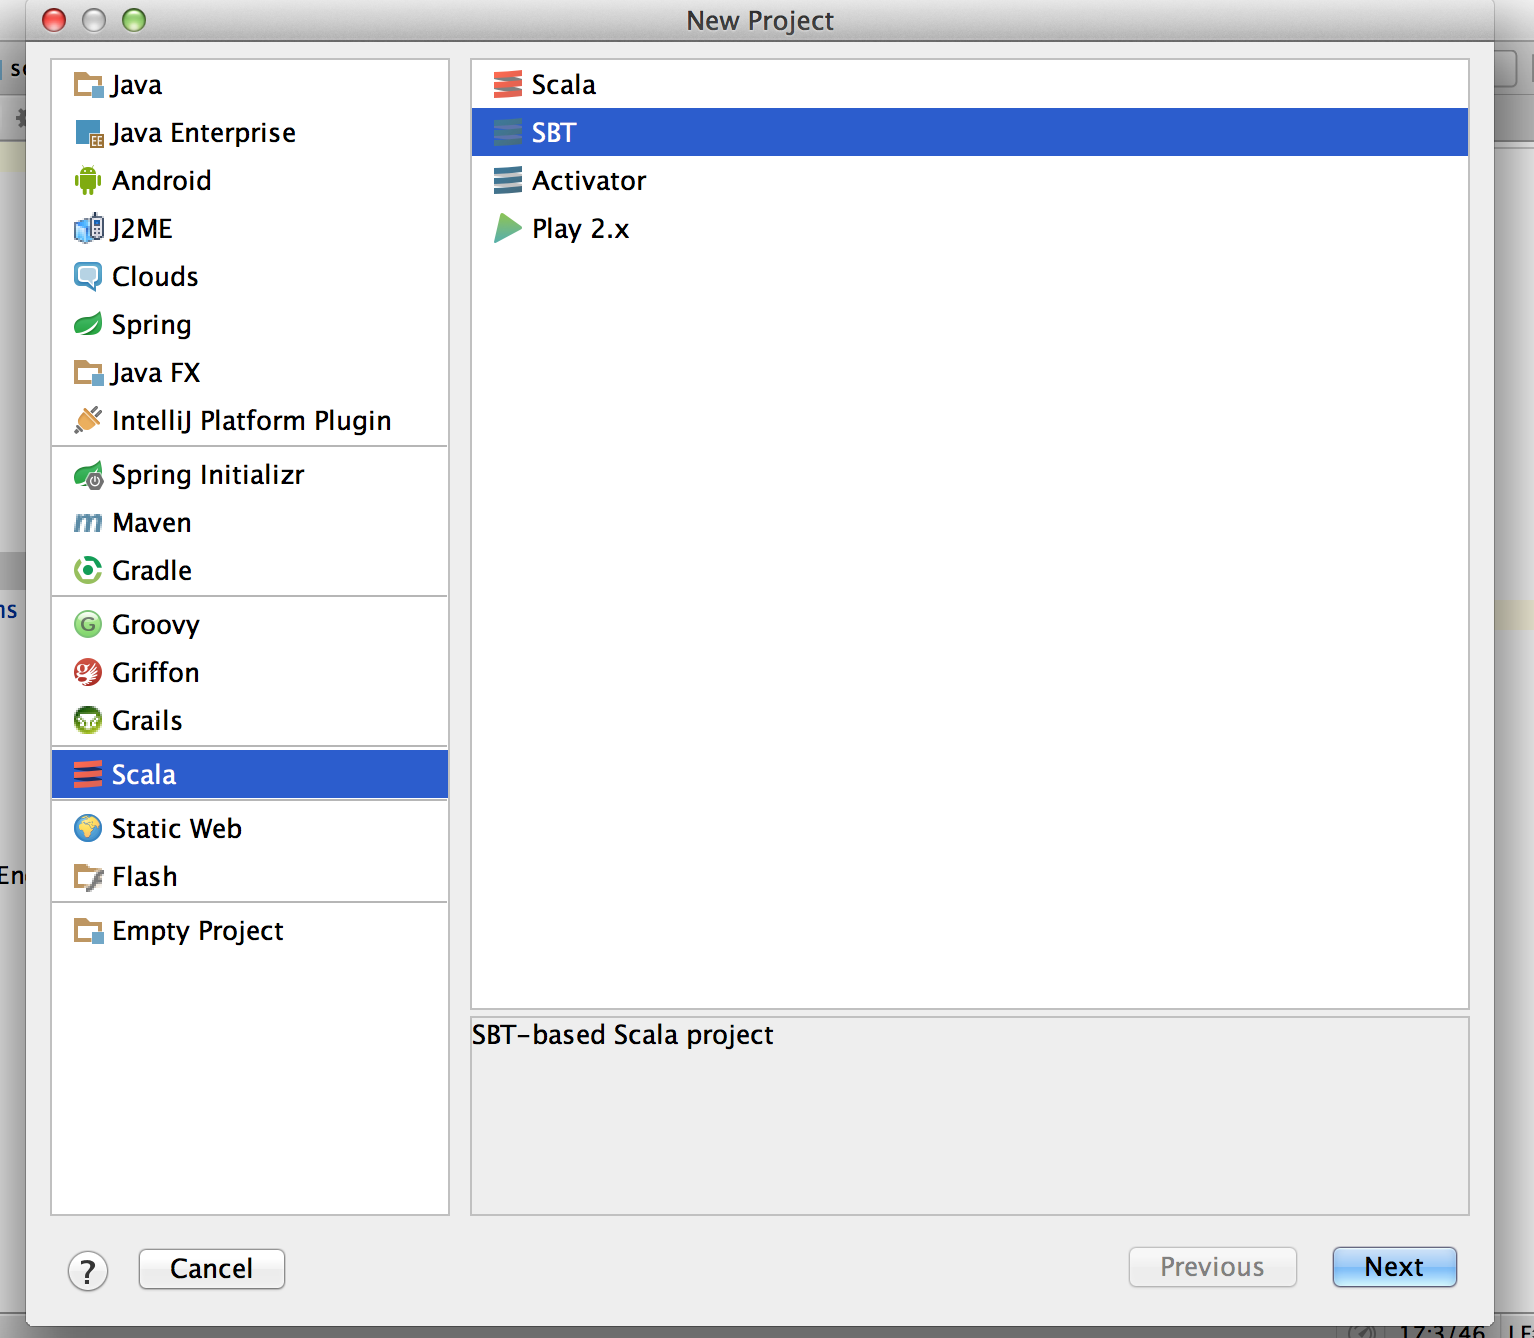
\includegraphics[width=7in, height=4in, keepaspectratio=true, trim=0em 3em 0em 3em]{img1.png}
\end{center}
\vspace{0.5cm}

Go ahead and click Next. To simplify things, go ahead and check the four boxes corresponding to the options : Use auto-import, Create directories for empty content roots automatically, Download sources and docs, Download SBT sources and docs. Save this project in a desired directory, and click Finish. For illustration purposes, we will assume this project is saved in a project directory called TextManipulationEngine.

The new project should now be initialized. Expand the \enquote{project} directory in your sidebar (shown below)

\begin{center}
\vspace{0.6cm}
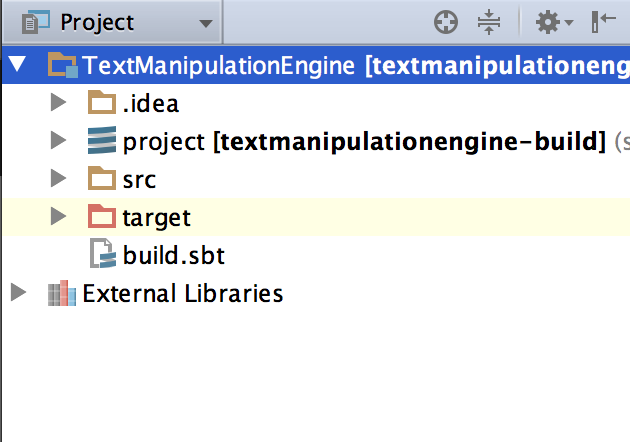
\includegraphics[width=3in, height=2in, keepaspectratio=true, trim=0em 3em 0em 3em]{img2.png}
\end{center}
\vspace{0.5cm}


Upon expanding, you should see four different items. Go ahead and select the files \tt{build.properties} and \tt{plugins.sbt}, right-click and select Delete as we will not be needing these files. Now, right-click on the main project directory (corresponding to the symbol consisting of three blue lines), select New and then File. You will name this file \tt{assembly.sbt}. In this file you will include the line
$$
\tt{addSbtPlugin("com.eed3si9n" \% "sbt-assembly" \% "0.13.0")}
$$
You may need to change the version number (the string following the second \%) depending on what version of SBT you are using. Now, repeat the latter step, this time creating a file named \tt{pio-build.sbt}. In this file, you will include the line
$$
\tt{addSbtPlugin("io.prediction" \% "pio-build" \% "0.9.0")}
$$
Modify the version number as necessary. 

Alright, now we are ready to setup our \tt{build.sbt} file. Modify this to include only the following:
\begin{verbatim}
name := "TextManipulationEngine"

libraryDependencies ++= Seq(
  "io.prediction"    %% "core"        % pioVersion.value % "provided",
  "org.apache.spark" %% "spark-core"  % "1.2.0"          % "provided",
  "org.apache.spark" %% "spark-mllib" % "1.2.0"          % "provided"
)
\end{verbatim}
Again, modify version numbers as necessary. Now, recall that we will be using Apache's OpenNLP library for purposes of text manipulation. To include this, you will add the following line to your \tt{build.sbt} file:
$$
\tt{libraryDependencies += "org.apache.opennlp" \% "opennlp-tools" \% "1.5.3"}
$$
At this point, you should be able to compile your project. 

We are now ready to start developing our engine, but first we will download some data which we will be using to test our engine. This is the subject of the following section.

\section*{Import Data}

For illustration purposes, we will be using the data available for the following Kaggle competition:
$$
\tt{https://www.kaggle.com/c/sentiment-analysis-on-movie-reviews/data}
$$
Create a directory in the TextManipulationEngine called \enquote{data.} Download the \tt{train.tsv} zip file from the Kaggle competition site, unzip the file, and place the resulting \tt{tsv} file in the data directory you just created. We now recall how your app will interact with our engine:

\begin{center}
\vspace{0.6cm}
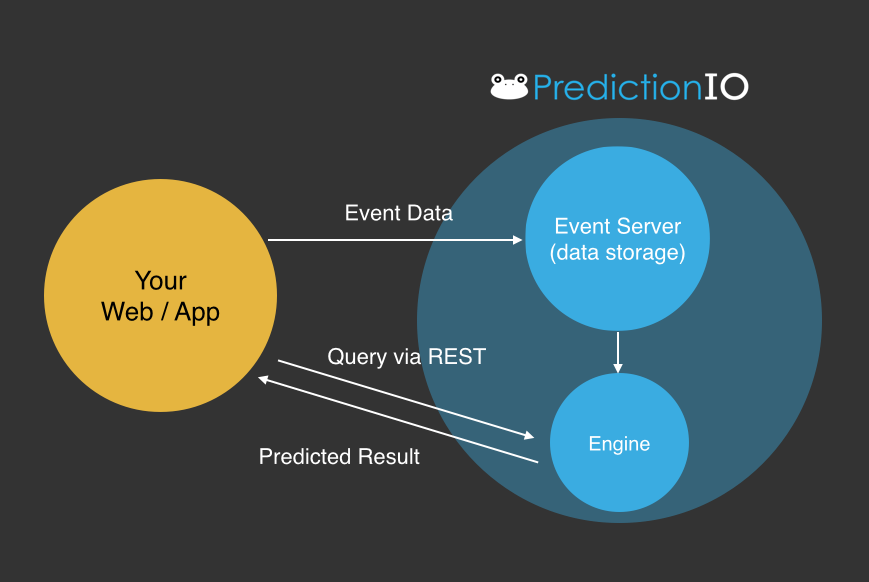
\includegraphics[width=4in, height=3in, keepaspectratio=true, trim=0em 3em 0em 3em]{img3.png}
\end{center}
\vspace{0.5cm}


As a user, we are charged with collecting data and importing it into an event server. The data will then be read and processed by our engine via the \tt{DataSource} and \tt{Preparation} components. The \tt{Algorithm} engine component then trains a predictive model using the processed, or prepared, data. Once we have trained a model, we are ready to deploy our engine and respond to real-time queries via the \tt{Serving} component.

In this section, we are dealing with the data collection process. The data we have collected is stored in \tt{train.tsv}. We will be using the PredictionIO Python SDK to import our data into PredictionIO's Event Server. Let's first explore our data a little bit more using our Terminal shell. First change into the TextManipulationEngine directory. From here using the command \tt{head -n 2 data/train.tsv}, we obtain in the following output, the first two lines of our data document:

\begin{verbatim}
PhraseId	SentenceId	Phrase	Sentiment
1	1	A series of escapades demonstrating the adage that what is good for the goose 
is also good for the gander , some of which occasionally amuses but none of which 
amounts to much of a story .	1
\end{verbatim}

The first line gives us our variable names, and the second gives us the first observation of our data. We will take note of the variable names, but use the command 
$$
\tt{sed -e "1d" data/train.tsv > x; mv x data/train.tsv}
$$ 
to remove the first line from the document to avoid complications when reading the data later.  We also note that each observation's data entry is separated by a  $\backslash\tt{t}$ character. We are now ready to import our data into the event server. 

Our main tool from the Python SDK that we will use to import our data into the event server is the class \tt{EventClient} and its method \tt{create\_event}. Now, in your data directory create a file named \tt{import\_eventserver.py}. Initialize the script by adding the following lines:
\begin{verbatim}
import predictionio
import argparse
\end{verbatim}
We will now define a function \tt{import\_events} which will take as input an object of type \tt{EventClient} and a string object providing the name of the data document, which is in our case \tt{train.tsv}. We will skip the details of the document processing in Python, and refer to the reader to the following documentation:
$$
\tt{https://docs.python.org/2/library/strings.html}
$$
We will process each line in the file and convert it to a list of strings. Once each line is processed, an event is created using the aforementioned client method. We will be assigning various properties to our data so that our engine can successfully read the corresponding event data parts that will be needed to train our predictive model. Your function should look similar to the following:
\begin{verbatim}
def import_events(client, file):
    f, count = open(file, 'r'), 0
    print("Importing data...")
    for line in f:
        count += 1
        line = line.replace('\n', '').split('\t')
        client.create_event(
            event = "text",
            entity_id = line[0],
            entity_type = "user",
            properties = {
                "text" : line[2],
                "label" : line[3],
            }
        )
    f.close()
    print("Imported {0} events.".format(count))
\end{verbatim}

In the latter function we save as event properties the actual text data itself, and the classification label associated to it. In the future, it will be easier to abstract our learning predictors/features as simply strings of text. Also, since we are storing as an event property a label associated to each string, we can both illustrate supervised training (classification) and unsupervised training (clustering) with this text data.

\break

The library \tt{argparse} is a Python module used to read in arguments from the command line. In this tutorial, this will be used when we want to enter the appropriate access key for our application. The remaining code for our Python script sets these arguments settings, and initializes an \tt{EventClient} instance, and finally calls our \tt{import\_event} function on the client instance and the given file argument.

\begin{verbatim}
if __name__ == '__main__':
    parser = argparse.ArgumentParser(
        description="Import sample data for text manipulation engine")
    parser.add_argument('--access_key', default='invald_access_key')
    parser.add_argument('--url', default="http://localhost:7070")
    parser.add_argument('--file', default="./data/train.tsv")

    args = parser.parse_args()

    client = predictionio.EventClient(
        access_key=args.access_key,
        url=args.url,
        threads=5,
        qsize=500)

    import_events(client, args.file)
\end{verbatim}

Awesome! Now, we are ready to import our data into PredictionIO's Event Server. To do this, using Terminal, go to the TextManipulationEngine directory. First, to avoid any errors due to currently running instances, go ahead and type in the command \tt{pio-stop-all}. Now, restart the process by typing \tt{pio-start-all}, and create a new application by typing in the command \tt{pio app new TextApp1}. You should see set of lines of output of the form
\begin{verbatim}
[INFO] [App$] Initialized Event Store for this app ID: 5.
[INFO] [App$] Created new app:
[INFO] [App$]       Name: TextApp1
[INFO] [App$]         ID: 5
[INFO] [App$] Access Key: *****
\end{verbatim}
Take note of your access key. Now, run the following command to begin importing events:
$$
\tt{python data/import\_eventserver.py --access\_key *****}
$$
This part may take a little while, but if the data is successfully loaded you should see the following printed output:
\begin{verbatim}
Importing data...
Imported 156060 events.
\end{verbatim}

We will now go ahead and begin integrating the OpenNLP library for use in our engine. 

\break

\section*{Integrating OpenNLP and Building a Text Processing Toolset}

Currently each observation $x$ in our data can be expressed in the form $(y_x, D_x)$ where $y_x$ is a discrete variable, and $D_x,$ some string, or document. We cannot yet perform a learning algorithm on the document data in its current representation, as we must first transform it to an appropriate numeric representation. The simplest model to do this is to assume each document $D_x$ is of the form
$$
\text{token}_{x, 1} \ \ \text{token}_{x, 2} \ \ \cdots \ \ \text{token}_{x, m_x}.
$$
These tokens can be words, punctuation symbols, or even single characters. In the case of our sample data, we are dealing with phrases and sentences which perfectly match this form. The two representations of our text data matrix that we will use for training in this tutorial are based on the following construction.

We will let $\mathcal{V},$ our vocabulary, denote the set of all tokens appearing in our data documents. For any practical application, this set will be finite, and so we can assume some arbitrary indexing by integers on our tokens $t_1, ..., t_{|\mathcal{V}|}.$ Now, we can associate to our vocabulary a real vector space of dimension $|\mathcal{V}|$ by assigning the $i^\text{th}$ standard basis vector to the $i^\text{th}$ token in the vocabulary $\3(\text{for those algebraists out there, this is simply the free $\R$-module over $\mathcal{V}$}\4).$ This construction allows us to represent our documents as vectors in this vector space! 

Of course, in order to even begin implementing anything relating to the latter construction, we need to be able to tokenize each of our documents. Let's start by creating a class called \tt{TextVectorizer} and defining a private method called \tt{tokenize}. We will use OpenNLP's \tt{SimpleTokenizer} class to do this, which can be imported with the statement \tt{import opennlp.tools.tokenize.SimpleTokenizer}. We note that there are other choices available in the OpenNLP library for tokenizers if you wishes to explore a more fitting option for your needs.


To do this, we can easily define a function \tt{tokenize} that takes in a document (or sentence represented as type \tt{String} in Scala), and returns an array of tokens in the order that they appear in the document. 

\subsection*{Bag-of-Words Model}

In this model, we want to transform each document $D$ into a collection of pairs $(t, n_t)$ where $t$ denotes a unique token appearing in $D,$ and $n_t$ the number of counts it appears in the document. We will then embed $D$ as a vector with entry $n_t$ corresponding the basis vector associated to the token $t$, and 0 for all entries corresponding to tokens not present in $D.$ For example, say that my 







\end{document}